\documentclass[10pt]{article}
\usepackage{tikz}
\usetikzlibrary{shapes.misc}
\usepackage[margin=0cm]{geometry}
\pagestyle{empty}
\tikzstyle{every node}=[cross out, draw, red]

\begin{document}

\vspace*{\fill}
\begin{center}
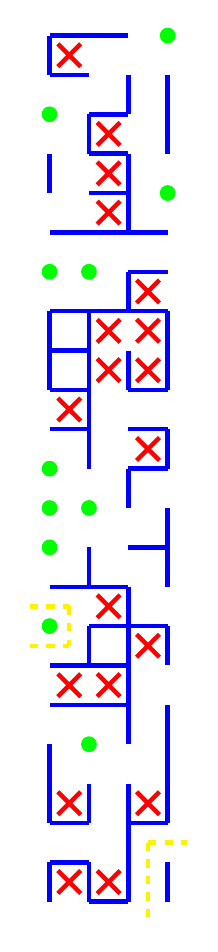
\begin{tikzpicture}[x=0.5cm, y=-0.5cm, ultra thick, blue]
% Walls
    \draw (0,0) -- (2,0);
    \draw (0,1) -- (1,1);
    \draw (1,2) -- (2,2);
    \draw (1,3) -- (2,3);
    \draw (1,4) -- (2,4);
    \draw (0,5) -- (3,5);
    \draw (2,6) -- (3,6);
    \draw (0,7) -- (3,7);
    \draw (0,8) -- (1,8);
    \draw (0,9) -- (1,9);
    \draw (2,9) -- (3,9);
    \draw (0,10) -- (1,10);
    \draw (2,10) -- (3,10);
    \draw (2,11) -- (3,11);
    \draw (2,13) -- (3,13);
    \draw (0,14) -- (2,14);
    \draw (1,15) -- (3,15);
    \draw (0,16) -- (2,16);
    \draw (0,17) -- (2,17);
    \draw (0,20) -- (1,20);
    \draw (2,20) -- (3,20);
    \draw (0,21) -- (1,21);
    \draw (1,22) -- (2,22);
    \draw (0,0) -- (0,1);
    \draw (0,3) -- (0,4);
    \draw (0,7) -- (0,9);
    \draw (0,18) -- (0,20);
    \draw (0,21) -- (0,22);
    \draw (1,2) -- (1,3);
    \draw (1,7) -- (1,11);
    \draw (1,13) -- (1,14);
    \draw (1,15) -- (1,16);
    \draw (1,19) -- (1,20);
    \draw (1,21) -- (1,22);
    \draw (2,1) -- (2,2);
    \draw (2,3) -- (2,5);
    \draw (2,6) -- (2,7);
    \draw (2,8) -- (2,9);
    \draw (2,11) -- (2,12);
    \draw (2,14) -- (2,18);
    \draw (2,19) -- (2,22);
    \draw (3,1) -- (3,3);
    \draw (3,7) -- (3,9);
    \draw (3,10) -- (3,11);
    \draw (3,12) -- (3,14);
    \draw (3,15) -- (3,16);
    \draw (3,17) -- (3,20);
    \draw (3,21) -- (3,22);
% Pillars
    \fill[green] (3,0) circle(0.2);
    \fill[green] (0,2) circle(0.2);
    \fill[green] (3,4) circle(0.2);
    \fill[green] (0,6) circle(0.2);
    \fill[green] (1,6) circle(0.2);
    \fill[green] (0,11) circle(0.2);
    \fill[green] (0,12) circle(0.2);
    \fill[green] (1,12) circle(0.2);
    \fill[green] (0,13) circle(0.2);
    \fill[green] (0,15) circle(0.2);
    \fill[green] (1,18) circle(0.2);
% Inner points in accessible cul-de-sacs
    \node at (0.5,0.5) {};
    \node at (1.5,2.5) {};
    \node at (1.5,3.5) {};
    \node at (1.5,4.5) {};
    \node at (2.5,6.5) {};
    \node at (1.5,7.5) {};
    \node at (2.5,7.5) {};
    \node at (1.5,8.5) {};
    \node at (2.5,8.5) {};
    \node at (0.5,9.5) {};
    \node at (2.5,10.5) {};
    \node at (1.5,14.5) {};
    \node at (2.5,15.5) {};
    \node at (0.5,16.5) {};
    \node at (1.5,16.5) {};
    \node at (0.5,19.5) {};
    \node at (2.5,19.5) {};
    \node at (0.5,21.5) {};
    \node at (1.5,21.5) {};
% Entry-exit paths without intersections
    \draw[dashed, yellow] (-0.5,14.5) -- (0.5,14.5);
    \draw[dashed, yellow] (-0.5,15.5) -- (0.5,15.5);
    \draw[dashed, yellow] (2.5,20.5) -- (3.5,20.5);
    \draw[dashed, yellow] (0.5,14.5) -- (0.5,15.5);
    \draw[dashed, yellow] (2.5,20.5) -- (2.5,22.5);
\end{tikzpicture}
\end{center}
\vspace*{\fill}

\end{document}
